\documentclass[border=5pt]{standalone}
\usepackage{tikz}
\usepackage{amsmath}
\usetikzlibrary{calc}
\begin{document}
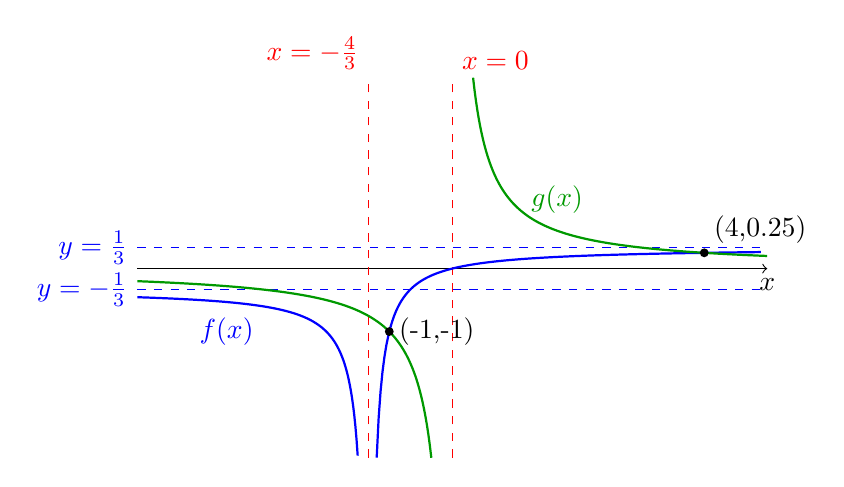
\begin{tikzpicture}[scale=0.8]
    % Axes
    \draw[->] (-5,0) -- (5,0) node[below] {$x$};

    % Vertical asymptotes
    \draw[dashed, red] (-4/3,-3) -- (-4/3,3) node[above left] {$x=-\frac{4}{3}$};
    \draw[dashed, red] (0,-3) -- (0,3) node[above right] {$x=0$};
    \draw[dashed, blue] (-5,1/3) -- (5,1/3);
    \node[left, blue] at (-5,1/3) {$y=\frac{1}{3}$};
    \draw[dashed, blue] (-5,-1/3) -- (5,-1/3);
    \node[left, blue] at (-5,-1/3) {$y=-\frac{1}{3}$};

    % f(x) plot components
    \draw[blue, thick, domain=-5:-1.5, samples=200] plot (\x, {\x/(-(3*\x +4))});
    \draw[blue, thick, domain=-1.2:4.9, samples=200] plot (\x, {\x/(3*\x +4)});
    \node[blue, left] at (-3,-1) {$f(x)$};

    % g(x) plot
    \draw[green!60!black, thick, domain=-5:-0.33, samples=200] plot (\x, {1/\x});
    \draw[green!60!black, thick, domain=0.33:5, samples=200] plot (\x, {1/\x});
    \node[green!60!black, right] at (1.1,1.1) {$g(x)$};

    % Intersection points
    \fill (-1,-1) circle (2pt) node[right] {(-1,-1)};
    \fill (4,0.25) circle (2pt) node[above right] {(4,0.25)};

\end{tikzpicture}
\end{document}
